\documentclass[conference]{IEEEtran}
\IEEEoverridecommandlockouts
\usepackage{cite}
\usepackage{amsmath,amssymb,amsfonts}
\usepackage{graphicx}
\usepackage{textcomp}
\usepackage{xcolor}
\usepackage{booktabs}
\usepackage{array}
\usepackage{url}
\def\UrlBreaks{\do\/\do-\do.\do_}
\usepackage[hidelinks]{hyperref}
\def\BibTeX{{\rm B\kern-.05em{\sc i\kern-.025em b}\kern-.08em
    T\kern-.1667em\lower.7ex\hbox{E}\kern-.125em X}}
\newcommand{\apcr}{\mathrm{APCR}}
\renewcommand{\arraystretch}{1.12}

\begin{document}

\title{Automatic API Security Design Review for Microservices Using Threat Graph Analysis}

\author{\IEEEauthorblockN{Phanapon Maneechot, Atiwat Thanapatsiri, Hiran Sanguantam, Sunya Nuchapong, Somchart Fugkeaw}
\IEEEauthorblockA{Sirindhorn International Institute of Technology, Thammasat University, Thailand\\
6622780326@g.siit.tu.ac.th, 6622780334@g.siit.tu.ac.th, 6622770632@g.siit.tu.ac.th, 6622782637@g.siit.tu.ac.th,\\
somchart@siit.tu.ac.th}}

\maketitle

\begin{abstract}
Microservice applications expose many internal and public APIs whose security depends on how services, gateways and deployment settings fit together. Existing tools look at one layer at a time: scanners read manifests or source code, API linters read specifications, and active scanners probe the endpoints listed in a specification. None of them answers the design question of which API weaknesses an outside attacker can actually reach, and commercial runtime platforms require production traffic to leave the organization. This paper presents a self-hosted platform for automatic API security design review that runs next to a test deployment and never exports data. It combines four evidence sources (runtime traffic captured by a sidecar, OpenAPI documents, Kubernetes, Docker Compose and gateway configuration, and OpenTelemetry traces) into an Extended Universal JSON Format (EUJF) inventory. It evaluates 27 deterministic rules mapped to the OWASP API Security Top 10, builds a typed threat graph, and ranks attack paths with an Attack-Path-Aware Contextual Risk (APCR) score. A greedy planner orders the fixes, and a hardening report gives each fix in the technology the system uses. We evaluate the platform on 23 systems: three testbeds with an oracle ground truth, ten generated companies with planted weaknesses and negative controls, and ten published open-source systems with 716 labelled weaknesses. Combining the four sources finds 97--100\% of observable endpoints at a precision of 1.00, against 58--96\% for any single source. On the open-source systems the platform finds 65\% of the labelled weaknesses on all ten systems, while the best of eight free tools finds 46\% and runs on seven. The platform raises no alarm on 23 negative controls, and applying its fixes to the demonstration system removes 97\% of the attack-path risk.
\end{abstract}

\begin{IEEEkeywords}
API security, microservices, threat modeling, attack graph, API discovery, OWASP API Security Top 10, security design review.
\end{IEEEkeywords}

\section{Introduction}
Modern software systems rely on application programming interfaces (APIs) to connect services, databases and external partners. Microservice and cloud-native architectures multiply the number of APIs: one application may run dozens of services that call each other across a service mesh, behind one or more gateways. The OWASP API Security Top 10 lists the weaknesses that follow from this growth, such as broken object level authorization, broken authentication and improper inventory management \cite{owasp_api_2023}. NIST guidance for microservice systems recommends authenticating every service-to-service call, enforcing policy at the gateway and segmenting the network \cite{nist_800_204,nist_800_207}.

Whether a system meets these recommendations is a property of its design: which endpoints are public, which gateway routes require a token, which services accept calls from any pod, and which data each endpoint returns. This information is spread over several artefacts. API documents describe what the developers intended. Runtime traffic shows what is actually served, including endpoints nobody documented. Kubernetes manifests, Docker Compose files and gateway configurations decide what is exposed and how. Distributed traces reveal which service calls which. Each existing class of tool reads one of these artefacts. Configuration scanners such as Checkov, Kubescape and Polaris read manifests but know nothing about API behaviour \cite{checkov,kubescape,polaris}. API linters such as Spectral read specifications that are often incomplete \cite{spectral}. Static code scanners read one programming language each \cite{bandit,gosec,njsscan}. Active scanners such as OWASP ZAP send attack payloads to the endpoints listed in a specification \cite{zap}. Commercial API security platforms combine discovery with runtime protection, but they need production traffic to flow to the vendor's cloud or through the vendor's gateway \cite{ibm_apic,salt,akamai_api}.

Enterprises therefore face two problems. First, no single artefact gives a complete and correct picture of the API surface, so a review based on one source misses shadow endpoints, misreads authentication and cannot follow an attack across services. Second, the data that would close the gap (source code, traffic, traces) is often confidential and cannot be sent to an external service.

This paper addresses both problems with a locally deployed design-review platform, which we call ATG (API Threat Graph). ATG runs as a second Docker deployment attached to the network of the system under review. It captures traffic through a sidecar proxy, receives traces through an OpenTelemetry Collector, probes API documents and reads the deployment files read-only. It keeps all evidence in memory and deletes it after the review. We study four research questions:
\begin{itemize}
\item \textbf{RQ1:} Does combining four evidence sources discover and reconcile the API inventory better than any single source?
\item \textbf{RQ2:} Is the threat model built from extracted evidence accurate, and how does it compare with configuration scanners, API linters, code scanners and an active scanner?
\item \textbf{RQ3:} Does the attack-path-aware risk score lead to fixes that reduce risk in practice?
\item \textbf{RQ4:} How large a system can the analysis handle, and what can a passive review not detect?
\end{itemize}

The main contributions are:
\begin{enumerate}
\item \textit{A privacy-preserving multi-source extractor} that combines runtime traffic, OpenAPI documents, deployment and gateway configuration (Kubernetes, Docker Compose, Kong, nginx, Spring Cloud Gateway, Zuul, Istio) and distributed traces, without access to source code and without data leaving the client's environment.
\item \textit{The Extended Universal JSON Format (EUJF)}, which joins evidence about each operation across sources, keeps its provenance, and classifies the inventory as documented, shadow, zombie or dormant.
\item \textit{A threat graph with Attack-Path-Aware Contextual Risk (APCR)}: 27 deterministic rules mapped to OWASP, CWE, MITRE ATT\&CK and NIST, six node types, a recursive attack-path query in the graph store, risk propagation, and a greedy remediation planner with a hardening report that writes each fix for the technology the system uses.
\item \textit{An evaluation on 23 systems}: three testbeds scored against an oracle built from ground truth, ten generated companies with planted weaknesses and negative controls, and ten published open-source systems from nine domains. On the open-source systems we compare ATG with eight free tools and, on the demonstration system, with OWASP ZAP.
\end{enumerate}

The rest of the paper is organized as follows. Section~\ref{sec:related} reviews related work. Section~\ref{sec:system} describes the platform. Section~\ref{sec:setup} describes the experimental setup, and Section~\ref{sec:eval} reports the evaluation. Section~\ref{sec:discussion} discusses limitations and threats to validity, and Section~\ref{sec:conclusion} concludes.

\section{Related Work}\label{sec:related}
\subsection{API security testing and runtime protection}
Research in API security and microservice assessment spans vulnerability classification, runtime intrusion detection and formal contract modeling. Abdurrahman and Husni evaluated countermeasures against the OWASP API Security Top 10 in a Spring Boot marketplace \cite{r1}. Their findings confirmed that parameter tampering, BOLA and excessive resource consumption can be mitigated by centralized gateway filtering, data transfer object binding and declarative route constraints, but the verification focused on single-service implementations and manual remediation. Idris et al. proposed the Vulnerable Academic Information System (VAIS), a testbed based on OWASP API security risks for dynamic testing and black-box penetration testing \cite{r2}. It relies on manual enumeration and does not automate design-time analysis.

George and Jonnalagadda placed a Random Forest threat detector at the API gateway that uses HTTP traffic logs and inter-arrival times to detect brute-force and injection attempts with low latency \cite{r3}. Sattanadin proposed an intelligent gateway framework that combines deterministic controls with machine learning over distributed traces and call graphs \cite{r5}, and Ratra et al. and Bhesaniya et al. studied AI-enhanced gateways and access-behaviour analysis \cite{r7,r8}. These approaches detect attacks at runtime, assume centralized telemetry, and do not evaluate structural configuration flaws before deployment. Tang et al. formalized API security with Object-Z and Design by Contract, which gives mathematical guarantees but requires manual state schemas for each service \cite{r4}. D\'iaz-Rojas et al. mapped 66 web API threats to STRIDE and observed that communication channels and authorization boundaries are the most targeted components \cite{r6}. Sun et al. showed that unowned and zombie APIs spread quickly in distributed environments and that single-host taint analysis fails across network boundaries \cite{r9}.

\subsection{Threat modeling tools}
Threat modeling decomposes a system into a data-flow diagram and applies a threat taxonomy such as STRIDE \cite{shostack}. The Microsoft Threat Modeling Tool generates STRIDE threats per interaction of a hand-drawn diagram \cite{ms_tmt}, and OWASP Threat Dragon suggests threats per diagram element \cite{threat_dragon}. Threagile evaluates about 40 risk rules over a model written in YAML \cite{threagile}, and IriusRisk generates threat models from Terraform or CloudFormation descriptions \cite{iriusrisk}. All of them start from a model that a person writes or that describes cloud infrastructure, so the model can drift from the running system. ATG builds the model from the running system and its deployment files.

\subsection{Commercial API security platforms}
IBM API Connect integrates Akamai (formerly Noname) API security for discovery, posture management, runtime protection and active testing of APIs managed by IBM's gateways \cite{ibm_apic}. Salt Security mirrors API traffic out of band for discovery and behavioural threat detection \cite{salt}. Akamai API Security discovers APIs from traffic, code repositories, documentation and gateways \cite{akamai_api}. Harness (Traceable) builds its picture from distributed traces collected by agents in each service \cite{traceable}. Wiz connects cloud resources, identities and exposure in a security graph with attack paths \cite{wiz}. Palo Alto Prisma Cloud discovers endpoints with agents or VPC mirroring \cite{prisma}, and Microsoft Defender for APIs covers APIs published in Azure API Management \cite{defender_apis}. 42Crunch audits OpenAPI contracts and tests running APIs against them \cite{crunch42}. NVIDIA Morpheus is a GPU framework for building AI detectors over streaming security data, such as digital fingerprinting and sensitive-information detection \cite{morpheus}. These products target production operation and require a subscription, a cloud account, the vendor's gateway or GPUs. We could not run them, and Table~\ref{tab:related} compares them from their documentation.

\subsection{Configuration, specification and code scanners}
Checkov, Kubescape, kube-linter and Polaris check Kubernetes manifests against best-practice policies \cite{checkov,kubescape,kubelinter,polaris}. Spectral lints OpenAPI documents, with an OWASP ruleset \cite{spectral}. Bandit, gosec and njsscan scan Python, Go and Node.js source \cite{bandit,gosec,njsscan}. Each reads one artefact type, and Section~\ref{sec:eval-b} measures what that means on ten real systems.

\begin{table*}[t]
\caption{Comparison with representative approaches (commercial tools from their public documentation)}
\label{tab:related}
\centering
\scriptsize
\setlength{\tabcolsep}{3pt}
\begin{tabular}{@{}p{3.3cm}>{\centering\arraybackslash}p{1.75cm}>{\centering\arraybackslash}p{2.0cm}>{\centering\arraybackslash}p{1.1cm}>{\centering\arraybackslash}p{2.0cm}>{\centering\arraybackslash}p{1.35cm}>{\centering\arraybackslash}p{1.35cm}>{\centering\arraybackslash}p{1.8cm}@{}}
\toprule
Approach & Runtime evidence & Deployment / gateway files & API documents & Attack graph & Before production & No data leaves & Ordered fixes \\
\midrule
Threat modeling tools \cite{ms_tmt,threat_dragon,threagile} & No & No & No & Per element & Yes & Yes & No \\
IriusRisk \cite{iriusrisk} & No & Cloud IaC & No & Rules on model & Yes & No (SaaS) & Countermeasures \\
K8s scanners \cite{checkov,kubescape,kubelinter,polaris} & No & K8s only & No & No & Yes & Yes & Per check \\
Spectral, 42Crunch \cite{spectral,crunch42} & Contract test & No & Yes & No & Yes & Partly & Per issue \\
OWASP ZAP \cite{zap} & Active probes & No & Yes & No & Yes & Yes & No \\
IBM API Connect + Akamai \cite{ibm_apic} & Gateway traffic & Gateway policy & Yes & Not stated & Testing & No & Posture \\
Salt, Akamai \cite{salt,akamai_api} & Mirrored traffic & Partly & Yes & Not stated & Partly & No & Posture \\
Harness Traceable \cite{traceable} & Traces (agents) & No & Yes & Call flows & CI tests & No & No \\
Wiz \cite{wiz} & Cloud APIs, eBPF & Cloud and K8s & No & Cloud-resource paths & Yes & No & Prioritized \\
Defender for APIs \cite{defender_apis} & APIM traffic & APIM only & Yes & Attack paths & No & No & Recommendations \\
NVIDIA Morpheus \cite{morpheus} & Streams, logs & No & No & No & No & Yes & No \\
\textbf{ATG (this work)} & \textbf{Traffic, traces} & \textbf{K8s, Compose, 5 gateways} & \textbf{Yes} & \textbf{API attack paths} & \textbf{Yes} & \textbf{Yes} & \textbf{Planned, per stack} \\
\bottomrule
\end{tabular}
\end{table*}

\section{Proposed System}\label{sec:system}
\subsection{System overview}
ATG is an on-premise, self-hosted review platform deployed next to the system under review with Docker Compose (Fig.~\ref{fig:arch}). It attaches to the system's Docker network and never needs its source code. Captured traffic, spans, intermediate files and the PostgreSQL graph store are held in memory (tmpfs volumes) and are deleted when the review stops; only the report pages and the exported graph are written to disk. The pipeline has four phases:
\begin{itemize}
\item \textbf{Phase 1, multi-source extraction:} four extractors collect runtime traffic, API documents, deployment and gateway configuration, and distributed traces.
\item \textbf{Phase 2, normalization:} the API normalizer merges the evidence into the EUJF inventory.
\item \textbf{Phase 3, analysis and risk assessment:} the dependency analyzer and the rule engine produce findings, which are compiled into a threat graph; attack paths are ranked with APCR and a planner orders the fixes.
\item \textbf{Phase 4, output:} a dashboard, an interactive threat graph, a hardening report and exports in GraphML, JSON, SARIF and SVG \cite{graphml,sarif}.
\end{itemize}

\begin{figure*}[t]
\centering
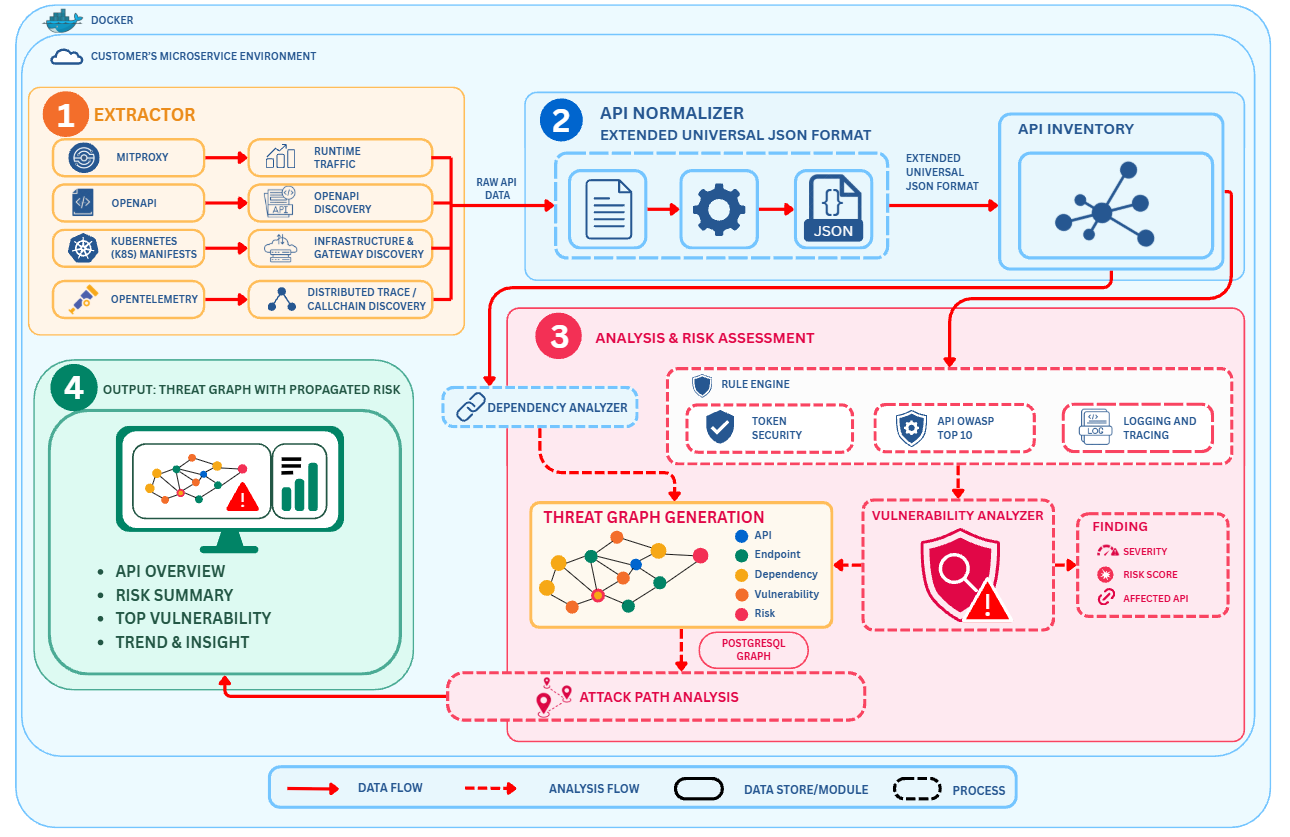
\includegraphics[width=0.86\textwidth]{figs/fig_architecture.png}
\caption{System architecture: four extractors (1), the API normalizer and EUJF inventory (2), analysis and risk assessment with the threat graph and attack-path analysis (3), and the output (4).}
\label{fig:arch}
\end{figure*}

\subsection{Phase 1: multi-source extractor}
\subsubsection{Runtime traffic (mitmproxy)}
A mitmproxy \cite{mitmproxy} sidecar runs in two modes: as a reverse proxy in front of the gateway (north-south traffic) and as a forward proxy for service-to-service calls (east-west traffic). It records method, path, status, headers that indicate credentials, and the shape of request and response bodies. It never stores secret values. Endpoints that are served but appear in no document become shadow candidates.

\subsubsection{OpenAPI discovery}
The extractor probes each service for a live document at common paths (\texttt{/openapi.json}, \texttt{/v3/api-docs}, \texttt{/swagger.json}, \texttt{/q/openapi} and others) and reads specification files from the repository. It extracts operations, parameters, request fields, declared security schemes and deprecation flags.

\subsubsection{Infrastructure and gateway discovery}
The extractor parses Kubernetes manifests (workloads, Services, Ingress, NetworkPolicy, Secrets, ConfigMaps), Istio resources (Gateway, VirtualService, AuthorizationPolicy, PeerAuthentication, EnvoyFilter), Docker Compose files, and gateway configurations of Kong, nginx, Spring Cloud Gateway and Netflix Zuul. It derives public entry points, routes with prefix stripping or rewriting, route-level authentication and rate limits, exposure through NodePort or LoadBalancer Services and published ports, TLS on each entry point, container security settings and plaintext secrets.

\subsubsection{Distributed traces (OpenTelemetry)}
An OpenTelemetry Collector \cite{otel} receives spans over OTLP, Zipkin and Jaeger. The extractor rebuilds call chains from parent--child relations and reports, for each endpoint, its callers and the traces that start at a backend without a traced caller. A call edge between services $S_A$ and $S_B$ is created when a client span of $S_A$ is the parent of a server span of $S_B$:
\begin{equation}
\mathrm{Span}_{\mathrm{parent}}(S_A,\mathit{op}_A) \xrightarrow{\ \mathrm{CALLS}\ } \mathrm{Span}_{\mathrm{child}}(S_B,\mathit{op}_B).
\label{eq:calls}
\end{equation}

\subsection{Phase 2: API normalizer and EUJF}
Raw observations contain concrete paths such as \texttt{GET /users/101} and \texttt{GET /users/102}. The normalizer replaces identifier segments (numbers, UUIDs and mixed tokens with a high digit share) with templates and reconciles the result with templates declared in API documents. Gateway traffic is mapped through the route table onto the backend operation, so one EUJF endpoint carries both its public path and its backend path. Fig.~\ref{fig:eujf} shows an EUJF record. Each record keeps the evidence of every source separately. The inventory status is \emph{documented} (in a document and observed), \emph{shadow} (observed, in no document), \emph{zombie} (deprecated in a document, still served) or \emph{dormant} (documented, never observed). Authentication is recorded as observed rather than as declared: it is \emph{enforced} when anonymous requests received 401 or 403 and none succeeded, and \emph{not enforced} when an anonymous request succeeded.

\begin{figure}[t]
\centering
\scriptsize
\begin{verbatim}
{ "id": "ep:order-service:GET:/orders/{order_id}",
  "service": "order-service", "method": "GET",
  "path": "/orders/{order_id}",
  "public_paths": ["/api/orders/{order_id}"],
  "inventory_status": "shadow",
  "auth_required": "enforced",
  "sources": {
    "traffic": {"calls": 42, "status": {"200": 40,
                                         "401": 2}},
    "trace":   {"spans": 42, "callers": ["api-gateway"]},
    "spec":    null },
  "data_classes": ["personal", "financial"],
  "object_id_in_path": true }
\end{verbatim}
\caption{An Extended Universal JSON Format (EUJF) endpoint record (abridged).}
\label{fig:eujf}
\end{figure}

\subsection{Phase 3: analysis and risk assessment}
\subsubsection{Dependency analyzer}
Service dependencies come from trace call edges \eqref{eq:calls}, from gateway routes, and from environment variables that name another service. Each dependency keeps its evidence.

\subsubsection{Rule engine and vulnerability analyzer}
The rule engine evaluates 27 deterministic rules over the EUJF in three groups: token security (8 rules), the OWASP API Security Top 10 (15 rules) and logging and tracing (4 rules). Each rule is a pure function of the EUJF, declares its OWASP 2023 category, CWE identifiers, MITRE ATT\&CK techniques \cite{attack,cwe} and NIST references \cite{nist_800_204,nist_800_207,nist_800_190,r10}, and carries base likelihood $L_0$ and impact $I_0$ values between 1 and 5. Table~\ref{tab:rules} lists representative rules. A finding's local risk is
\begin{gather}
R_{\mathrm{local}} = L \times I, \label{eq:local}\\
L = \mathrm{clip}_{[1,5]}\big(L_0 + \textstyle\sum_j \Delta L_j\big),\ \ I = \mathrm{clip}_{[1,5]}\big(I_0 + \textstyle\sum_k \Delta I_k\big), \nonumber
\end{gather}
where the adjustments $\Delta L_j$ and $\Delta I_k$ record context, for example $+1$ likelihood when the target is reachable from the internet, $-1$ when it is internal only, or $+1$ impact when the endpoint returns personal data. Every finding lists the adjustments that produced its score. Severity is critical for $R_{\mathrm{local}}\ge 20$, high for $\ge 12$, medium for $\ge 6$ and low otherwise.

\begin{table}[t]
\caption{Representative rules (27 in total)}
\label{tab:rules}
\centering
\footnotesize
\begin{tabular}{@{}p{1.35cm}p{4.35cm}cc@{}}
\toprule
Rule & Condition & $L_0$ & $I_0$ \\
\midrule
TS-01 & Sensitive operation answers anonymous callers & 4 & 4 \\
TS-02 & Gateway route forwards without authentication & 4 & 4 \\
TS-05 & Public entry serves the API without TLS & 3 & 4 \\
TS-06 & Credential passed in the URL query string & 3 & 4 \\
TS-07 & Login has no visible brute-force protection & 3 & 4 \\
TS-08 & Service-to-service call accepted without credentials & 2 & 4 \\
API1 & Possible BOLA: object ID in path, never a 403 & 3 & 4 \\
API5 & Administrative function reachable by ordinary callers & 4 & 5 \\
API7 & Request accepts a URL the server may fetch (SSRF) & 3 & 4 \\
API8-NETPOL & No network segmentation for the service & 2 & 3 \\
API9-SHADOW & Endpoint running but not documented & 3 & 3 \\
LT-01 & Calls from an unidentified internal caller & 3 & 3 \\
\bottomrule
\end{tabular}
\end{table}

\subsubsection{Threat graph generation}
Findings and the architecture are compiled into an attributed threat graph $G=(V,E,\Phi_V,\Phi_E)$ stored in PostgreSQL (or SQLite):
\begin{align}
V &= V_{\mathrm{Act}} \cup V_{\mathrm{API}} \cup V_{\mathrm{Ep}} \cup V_{\mathrm{Dep}} \cup V_{\mathrm{Vul}} \cup V_{\mathrm{Risk}}, \label{eq:v}\\
E &\subseteq V\times T_E\times V, \label{eq:e}\\
T_E &= \{\textsc{reaches},\textsc{exposes},\textsc{routes},\textsc{calls},\nonumber\\
 &\qquad \textsc{depends\_on},\textsc{runs\_on},\textsc{handles},\textsc{uses},\nonumber\\
 &\qquad \textsc{has\_vuln},\textsc{leads\_to}\}. \nonumber
\end{align}
Actors are the places an attack starts: the internet (an attacker who can register an ordinary account) and in-cluster code (a compromised pod). API nodes are services, endpoint nodes are operations, dependency nodes are data assets and credentials, vulnerability nodes are findings, and risk nodes are business consequences such as data breach, account takeover or financial fraud. \textsc{reaches} edges come from Ingress rules, NodePort and LoadBalancer Services, published ports, missing NetworkPolicies and untraced callers; \textsc{routes} edges from gateway routes; and \textsc{calls} edges from traces.

\subsubsection{Attack-Path-Aware Contextual Risk (APCR)}
An attack path $\pi=\langle a, v_1,\dots,v_k, f, r\rangle$ starts at an actor $a$, follows \textsc{reaches}, \textsc{routes}, \textsc{exposes} and \textsc{calls} edges, and ends at a finding $f$ and its risk $r$. Paths of up to nine hops are enumerated inside the database with a recursive common table expression, identical on SQLite and PostgreSQL. The risk of a path is
\begin{equation}
\apcr(\pi) = L(f)\times I(f)\times \varepsilon(a)\times \delta^{\,c(\pi)},
\label{eq:apcr}
\end{equation}
where $\varepsilon(a)=1.0$ for the internet actor and $0.5$ for the in-cluster actor (which first needs a foothold), $c(\pi)$ is the number of chained service-to-service calls on the path and $\delta=0.95$. APCR lies between 0 and 25. Paths are de-duplicated per (actor, first hop, finding). The total attack-path risk of the system sums, over all findings $F$, the best path that reaches each finding:
\begin{equation}
R = \sum_{f\in F}\ \max_{\pi\in\Pi(f)} \apcr(\pi).
\label{eq:r}
\end{equation}
A finding that no actor can reach adds nothing to $R$, however severe it is locally. Each node also receives a propagated risk, so that a gateway carries the risk of the worst thing it exposes:
\begin{equation}
\rho(n)=\max\Big(\mathrm{own}(n),\ \gamma\max_{m\in \mathrm{succ}(n)}\rho(m)\Big),\quad \gamma=0.85.
\label{eq:prop}
\end{equation}

\subsubsection{Remediation planner}
Findings are grouped into remediation actions, because one change often closes several findings (authentication plus a role check on an admin endpoint closes TS-01, API5 and API3 together). Two actions also remove edges: making a NodePort Service internal removes the internet \textsc{reaches} edge, and a NetworkPolicy removes the in-cluster one. The planner applies actions greedily:
\begin{equation}
a^{*}_t=\arg\max_{a\in A_t}\big(R_t - R_t\!\setminus\! a\big),
\label{eq:plan}
\end{equation}
where $R_t\!\setminus\! a$ is the total risk \eqref{eq:r} after removing the findings and edges of action $a$. The plan reports the risk left after each step and the number of fixes needed to remove 70\% and 90\% of $R$.

\subsection{Phase 4: output, hardening report and exports}
The dashboard shows the API inventory by source and status, the risk summary, the top findings, the trend across scans and the fix plan. The threat graph page (Fig.~\ref{fig:tg}) draws the graph by node type and lets the reviewer trace any ranked attack path. The hardening report (Fig.~\ref{fig:fixcard}) lists the planner's fixes in order. For each finding it gives the reason for its score, a fix written for the technology found in Phase 1 (for example a Kong, nginx, Spring Cloud Gateway or Istio route policy, a NetworkPolicy that admits exactly the callers seen in traces, or a code check naming the finding's own operation), a concrete test that verifies the fix, and its OWASP, CWE, ATT\&CK and NIST references. A per-service baseline marks each hardening control as present, missing or not observable. The graph is exported as GraphML, node-link JSON, SARIF 2.1.0 and SVG.

\begin{figure*}[t]
\centering
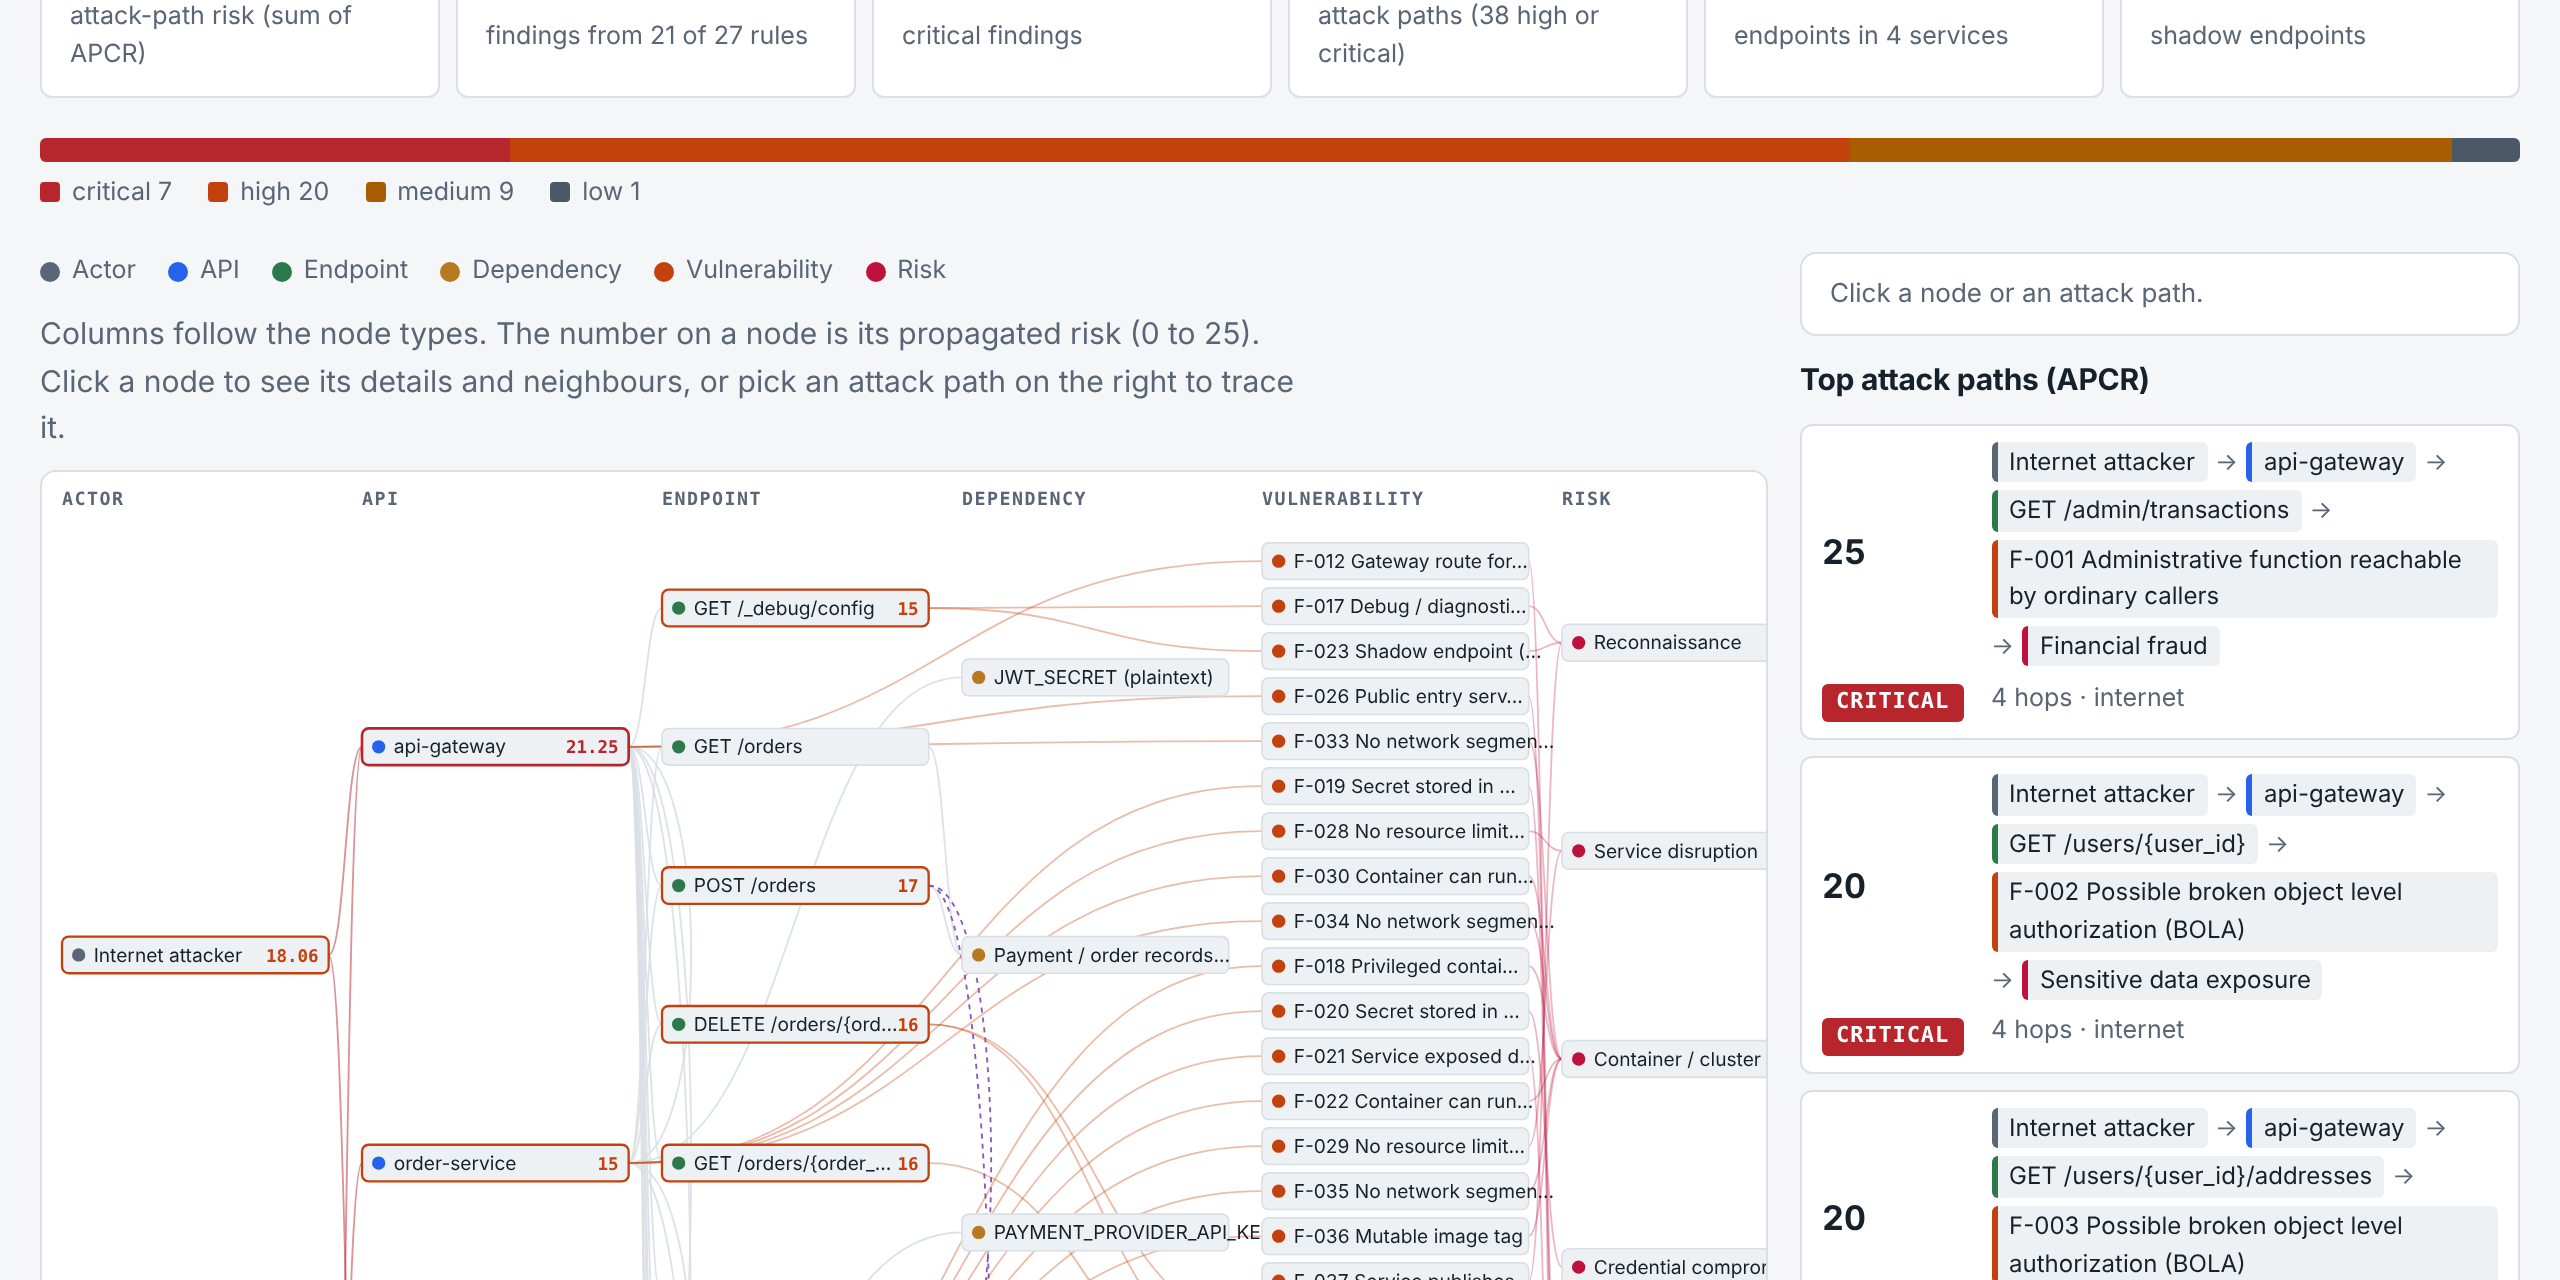
\includegraphics[width=0.95\textwidth]{figs/fig_threatgraph.png}
\caption{Threat graph output for the demonstration system (ShopLite, vulnerable build): summary, the graph by node type (actor, API, endpoint, dependency, vulnerability, risk) and the top attack paths ranked by APCR.}
\label{fig:tg}
\end{figure*}

\begin{figure}[t]
\centering
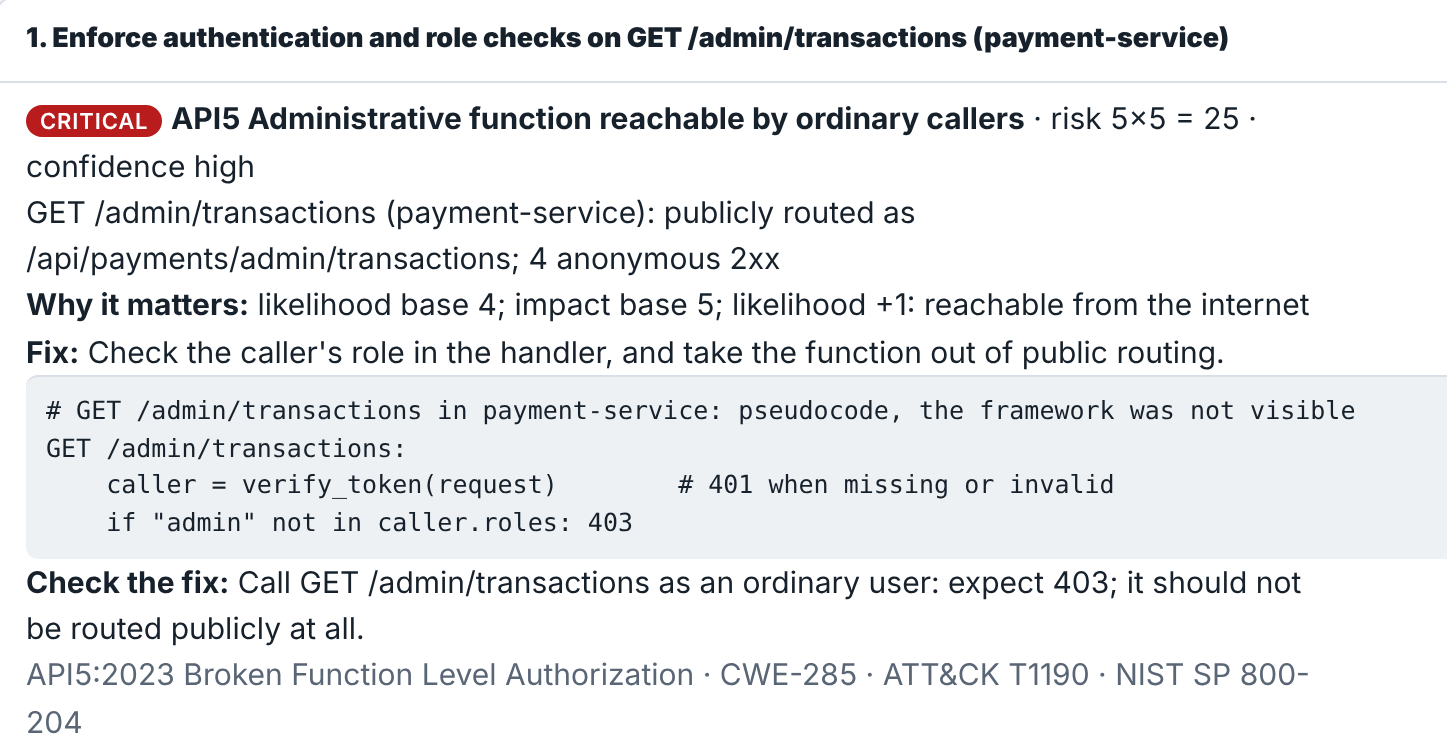
\includegraphics[width=\columnwidth]{figs/fig_fixcard.png}
\caption{One entry of the hardening report: the finding and its evidence, why it matters, the fix, a check that verifies it, and its references.}
\label{fig:fixcard}
\end{figure}

\section{Experimental Setup}\label{sec:setup}
\subsection{Implementation and environment}
ATG is implemented in Python (about 6,000 lines for the platform and 14,000 for the evaluation harness) and uses mitmproxy, the OpenTelemetry Collector (contrib 0.111.0) and PostgreSQL 16. All experiments ran on one Linux host with 2 vCPUs and 8 GB of memory. The code, the systems' definitions and every result file are in the project repository, together with scripts that rerun each experiment.

\subsection{Systems under test}
Table~\ref{tab:testbeds} summarizes the 23 systems in three groups.

\textit{Group A, oracle testbeds.} ShopLite is our demonstration shop of four FastAPI services with 12 endpoints and 40 planted weaknesses, three of which no rule covers; it has a vulnerable and a hardened build. Train Ticket (45 services, 272 endpoints) \cite{trainticket} and OWASP crAPI (6 services, 79 endpoints) \cite{crapi} run as API-surface replicas generated from their source code: each replica serves the mined routes, enforces the same authentication, makes the same downstream calls and emits traces, but returns generic bodies. Ground truth comes from the source code and from each service's own access log, which the extractors never read.

\textit{Group B, generated companies.} Ten companies in ten industries (fintech, hospital, airline, logistics, education, media, government, food delivery, insurance and telecom) differ in language (Go, Python, Node.js), gateway (Kong, nginx, Spring Cloud Gateway, Istio, a ConfigMap route table), login style and deployment habits. They contain 120 endpoints, 65 planted weaknesses and 23 negative controls, which look like weaknesses but are not.

\textit{Group C, open-source systems.} Ten published systems in nine domains, each pinned to one commit: Online Boutique and Bank of Anthos (Google) \cite{boutique,anthos}, Stan's Robot Shop and Acme Air (IBM) \cite{robotshop,acmeair}, Spring PetClinic \cite{petclinic}, PiggyMetrics \cite{piggymetrics}, Lakeside Mutual \cite{lakeside}, FTGO \cite{ftgo}, DeathStarBench Hotel Reservation \cite{deathstarbench} and Istio Bookinfo \cite{bookinfo}. They have 65 services in eight languages and 201 operations. Three are deployed with Docker Compose, five use a gateway (nginx, Spring Cloud Gateway, Zuul, an Ingress controller, routes in Java code), and five expose an edge service directly. ATG reads each system's own deployment files and API documents. Because the evaluation host could not pull container images, the running services are stand-ins built from each system's code, with the same names, ports, operations, call graph and authentication checks, answering with masked values.

\begin{table}[t]
\caption{Systems under test}
\label{tab:testbeds}
\centering
\footnotesize
\begin{tabular}{@{}p{2.1cm}rrp{3.25cm}@{}}
\toprule
Group & Systems & Endpoints & Ground truth \\
\midrule
A. Oracle testbeds & 3 & 363 & source code, access logs, oracle threat model; crAPI's OWASP list \\
B. Generated companies & 10 & 120 & 65 planted weaknesses, 23 negative controls \\
C. Open-source systems & 10 & 201 & 716 labels: 91 from code review, 625 by rule \\
\bottomrule
\end{tabular}
\end{table}

\subsection{Conditions and workload}
Group A runs under two conditions. Under \emph{C1 (ideal)} the sidecar captures north-south and east-west traffic and every service is traced. Under \emph{C2 (realistic)} only north-south traffic is captured and about 70\% of services are traced. The workload sends client sessions through the gateway that touch 80\% of public endpoints with Zipf-like popularity, 10\% of requests without a credential, and an in-cluster job that calls internal endpoints (3,000 requests per run for Train Ticket, 1,500 for crAPI). Five seeds per testbed and condition give 30 runs. Groups B and C run as the platform runs in practice: the system starts, its users send their requests through the sidecar, and ATG scans once.

\subsection{Ground truth and metrics}
\textit{Discovery.} An inventory entry matches a true endpoint when the method and the path shape agree. Recall over observable endpoints counts endpoints that are documented or received traffic, because no passive source can see the rest. Precision is strict: a second entry for the same endpoint is a false positive.

\textit{Threat model.} For Group A, an oracle EUJF is built from ground truth and the same Phase 3 code runs on it; a finding matches when rule and target agree. For Group B, a finding matches a planted weakness on the same rule and target. For Group C, each label is a weakness category on a service or an operation. 91 labels were written by reading the code, each with the source file, and 625 were derived by fixed rules from the deployment files, the call graph and the API documents. The categories fall into three groups: API behaviour (A1--A10), deployment configuration (C1--C10) and inventory and visibility (O1--O2). The findings of every tool are mapped to the same categories, and a label counts as found when the tool reports its category at the same place.

\subsection{Baselines}
On Group C we ran eight free tools on the same files: Checkov 3.4.5, Kubescape 3.0.18, kube-linter 0.7.1 and Polaris 9.6.1 on the Kubernetes manifests; Spectral 6.17.1 with the OWASP ruleset on the API documents; and Bandit 1.9.4, gosec 2.21.4 and njsscan 1.0.1 on the source code. As the active-scanner (DAST) baseline, OWASP ZAP 2.16.1 ran its default active-scan policy on ShopLite, once through the gateway and once inside the network, with the same API documents ATG used.

\section{Evaluation}\label{sec:eval}
\subsection{Endpoint Discovery and Reconciliation Performance}\label{sec:eval-a}
\textit{Combining sources.} Fig.~\ref{fig:discovery} compares single sources with all four under the realistic condition C2. Each single source misses a different part of the API: API documents miss shadow endpoints (61--68\% recall on ShopLite and crAPI), traffic misses endpoints that were not exercised (69\% on Train Ticket), and traces miss untraced services (58--74\%). All four together reach 97\%, 100\% and 97\% of observable endpoints with a precision of 1.00. Under the ideal condition C1, all four sources reach 100\% recall of observable endpoints on all three testbeds.

\begin{figure}[t]
\centering
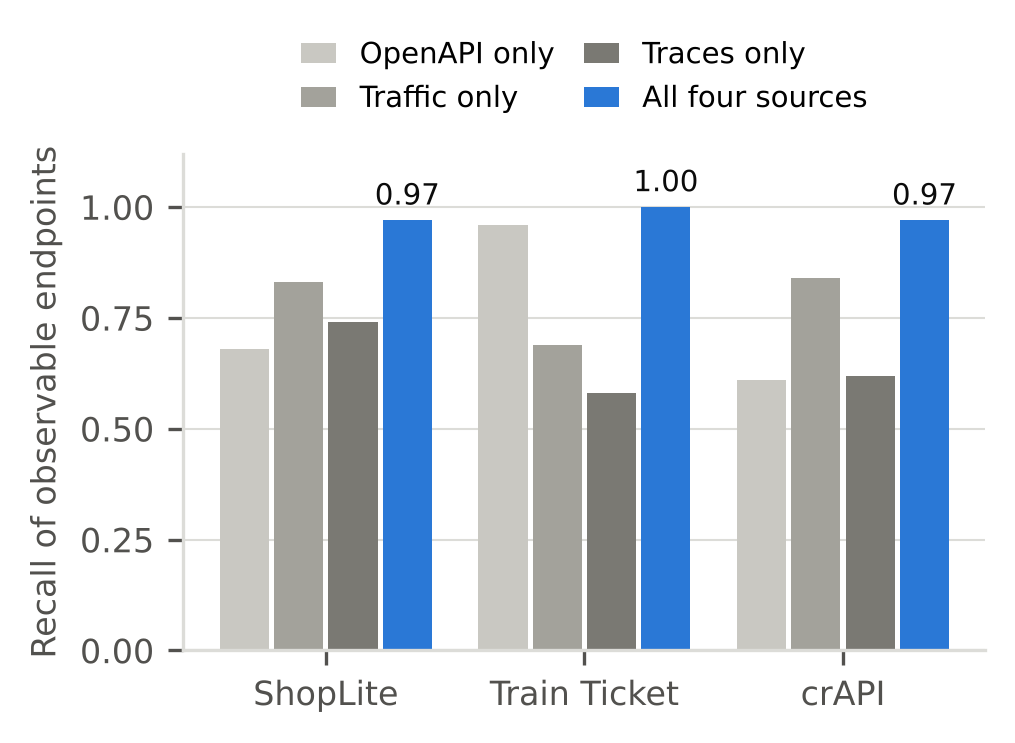
\includegraphics[width=\columnwidth]{figs/fig_discovery.png}
\caption{Endpoint recall of single sources and of all four sources together under the realistic condition C2 (mean of five seeds).}
\label{fig:discovery}
\end{figure}

\textit{Reconciliation.} Table~\ref{tab:recon} shows how raw observations collapse into the inventory. On Train Ticket under C1, 8,355 captured flows contain 1,383 distinct concrete paths. The single-source inventories hold 1,084 entries in total, and merging gives 264 entries after 821 duplicates are collapsed. Traffic alone leaves 228.6 fragments: entries whose path still holds a concrete value such as a station name. Reconciling with document templates removes all of them. Shadow endpoints are labelled with a precision of 1.00 in every run; their recall is 1.00 under C1 and 0.88--0.96 under C2. Authentication behaviour is classified correctly for every endpoint that received anonymous requests (accuracy 1.00).

\begin{table}[t]
\caption{Reconciliation of raw observations (condition C1, mean of five seeds)}
\label{tab:recon}
\centering
\footnotesize
\setlength{\tabcolsep}{3pt}
\begin{tabular}{@{}lrrr@{}}
\toprule
 & ShopLite & Train Ticket & crAPI \\
\midrule
Captured flows & 585 & 8,355 & 3,514 \\
Distinct concrete paths & 188 & 1,383 & 396 \\
Entries, single-source inventories & 41 & 1,084 & 262 \\
Entries after merging & 12 & 264 & 72 \\
Fragments, traffic only & 0 & 228.6 & 31.6 \\
Fragments, all four, reconciled & 0 & 0 & 0 \\
Shadow precision / recall & 1.00 / 1.00 & 1.00 / 1.00 & 1.00 / 1.00 \\
Dependency precision & 1.00 & 1.00 & 0.89 \\
Dependency recall (exercised) & 1.00 & 1.00 & 1.00 \\
\bottomrule
\end{tabular}
\end{table}

\textit{Dependencies.} Under C1, trace and gateway evidence together recover every exercised service dependency on all three testbeds, with a precision of 1.00, 1.00 and 0.89. Under C2, where 30\% of services send no spans, recall of exercised edges on Train Ticket falls to 0.77.

\textit{Generated and open-source systems.} On the ten generated companies ATG lists 120 of 120 endpoints with a precision of 100\%. On the ten open-source systems it lists 189 of 201 operations (94\%) with a precision of 88\%. The extra entries come from three systems: Acme Air, whose Ingress controller acts as the gateway for five services (15), FTGO, whose gateway routes are written in Java code that ATG does not read (8), and Bookinfo (4). ATG also found all 62 operations and services that have no API document and all 26 services that send no traces: 88 of 88 inventory and visibility labels.

\textit{Overhead.} The sidecar adds 3.0~ms (Train Ticket) and 3.4~ms (crAPI) to the median latency when it captures only north-south traffic, and 14.6--16.4~ms when it also carries east-west calls, with throughput falling from 147 to 113 requests per second on Train Ticket. Phase 1 takes 0.26~s on ShopLite and 1.25~s on Train Ticket.

\subsection{Threat Modeling Accuracy and Baseline DAST Comparison}\label{sec:eval-b}
\textit{Fidelity against the oracle.} Table~\ref{tab:oracle} compares the threat model built from extracted evidence with the oracle built from ground truth. With full visibility (C1) the two agree completely on all three testbeds: findings, attack paths, total risk $R$ and the ten highest-ranked findings. Under C2 the finding precision stays at 1.00 and recall falls to 0.82--0.94, mostly in rules that need east-west traffic (TS-08) or complete tracing (LT-01). An ablation over source subsets shows why all four are needed: the best three-source subset reaches a finding F1 of 0.80, 0.83 and 0.78 under C1, against 1.00 with all four.

\begin{table}[t]
\caption{Threat model built from extracted evidence vs.\ the oracle (C2, mean of five seeds; C1 gives 1.00 everywhere)}
\label{tab:oracle}
\centering
\footnotesize
\begin{tabular}{@{}lrrr@{}}
\toprule
 & ShopLite & Train Ticket & crAPI \\
\midrule
Finding precision & 1.00 & 1.00 & 1.00 \\
Finding recall & 0.82 & 0.88 & 0.94 \\
Finding F1 & 0.90 & 0.93 & 0.97 \\
Recall, critical and high & 0.77 & 0.80 & 0.99 \\
Attack-path recall & 0.86 & 0.87 & 0.93 \\
$R$ tool / $R$ oracle & 0.85 & 0.85 & 0.96 \\
Top-10 overlap (APCR rank) & 0.90 & 0.92 & 1.00 \\
\bottomrule
\end{tabular}
\end{table}

\textit{Known and planted weaknesses.} On ShopLite the rules find 36.6 of 40 planted weaknesses under C1 with a precision of 1.00; the three that no rule covers account for most of the gap. On the ten generated companies ATG finds 62 of 65 planted weaknesses (95\%), 62 of the 63 that a passive review can see, and 62 of its 64 findings are planted (97\%). Two misses were marked in advance as outside a passive review: an admin export that checks only that the caller is logged in, which passive traffic cannot tell from staff access, and a URL field named \texttt{photo\_url}, a name the SSRF rule does not know. The third is a claims export that ATG flags as anonymous and as bulk personal data (TS-01, API3) but not as an administrative function, because its path does not look like one. On OWASP's own list of 18 crAPI vulnerabilities, 12 are within reach of a passive tool at all; Section~\ref{sec:eval-e} discusses the rest.

\textit{Comparison with eight tools on ten open-source systems.} Table~\ref{tab:tools} and Fig.~\ref{fig:tools} compare ATG with the free tools against the same 716 labels. Only ATG reports API behaviour and inventory problems: 52 of 82 and 88 of 88 labels, against at most 10 and 0 for any other tool. On deployment configuration, ATG (60\%) is level with the best Kubernetes scanner, Polaris (61\%). The two check different things. ATG has no checks for container hardening (read-only file systems, dropped capabilities) or service-account tokens, which account for 169 labels. Polaris cannot read Docker Compose, so it skips three of the ten systems. Polaris is more precise (95\% against 75\%), because it checks exact manifest fields; many of ATG's unmatched reports are true but unlabelled, such as databases that send no traces.

\begin{table*}[t]
\caption{ATG and eight free tools on the ten open-source systems (716 labelled weaknesses). Times are from one run of the benchmark script on the 2-vCPU host; a whole ATG scan, including the wait for the capture buffers, takes 7.2--8.1~s.}
\label{tab:tools}
\centering
\footnotesize
\setlength{\tabcolsep}{4pt}
\begin{tabular}{@{}lrrrrrrr@{}}
\toprule
Tool & Runs on & Labels found & Configuration (546) & API behaviour (82) & Inventory (88) & Precision & Median time \\
\midrule
\textbf{ATG} & \textbf{10/10} & \textbf{466 (65\%)} & 326 (60\%) & \textbf{52 (63\%)} & \textbf{88 (100\%)} & 75\% & 0.35 s (Phases 1--4) \\
Polaris & 7/10 & 331 (46\%) & \textbf{331 (61\%)} & 0 & 0 & \textbf{95\%} & 0.13 s \\
Checkov & 7/10 & 262 (37\%) & 262 (48\%) & 0 & 0 & 74\% & 2.3 s \\
Kubescape & 7/10 & 254 (35\%) & 254 (47\%) & 0 & 0 & 87\% & 1.9 s \\
kube-linter & 7/10 & 164 (23\%) & 164 (30\%) & 0 & 0 & 89\% & 0.04 s \\
Spectral (OWASP ruleset) & 3/10 & 14 (2\%) & 4 & 10 (12\%) & 0 & 37\% & 1.4 s \\
Bandit / gosec / njsscan & 4/3/3 & 1 / 0 / 0 & 1 / 0 / 0 & 0 & 0 & 20\% / -- / -- & 0.47 / 3.6 / 0.61 s \\
\midrule
ATG + Checkov (either) & 10/10 & 613 (86\%) & & & & & \\
\bottomrule
\end{tabular}
\end{table*}

\begin{figure*}[t]
\centering
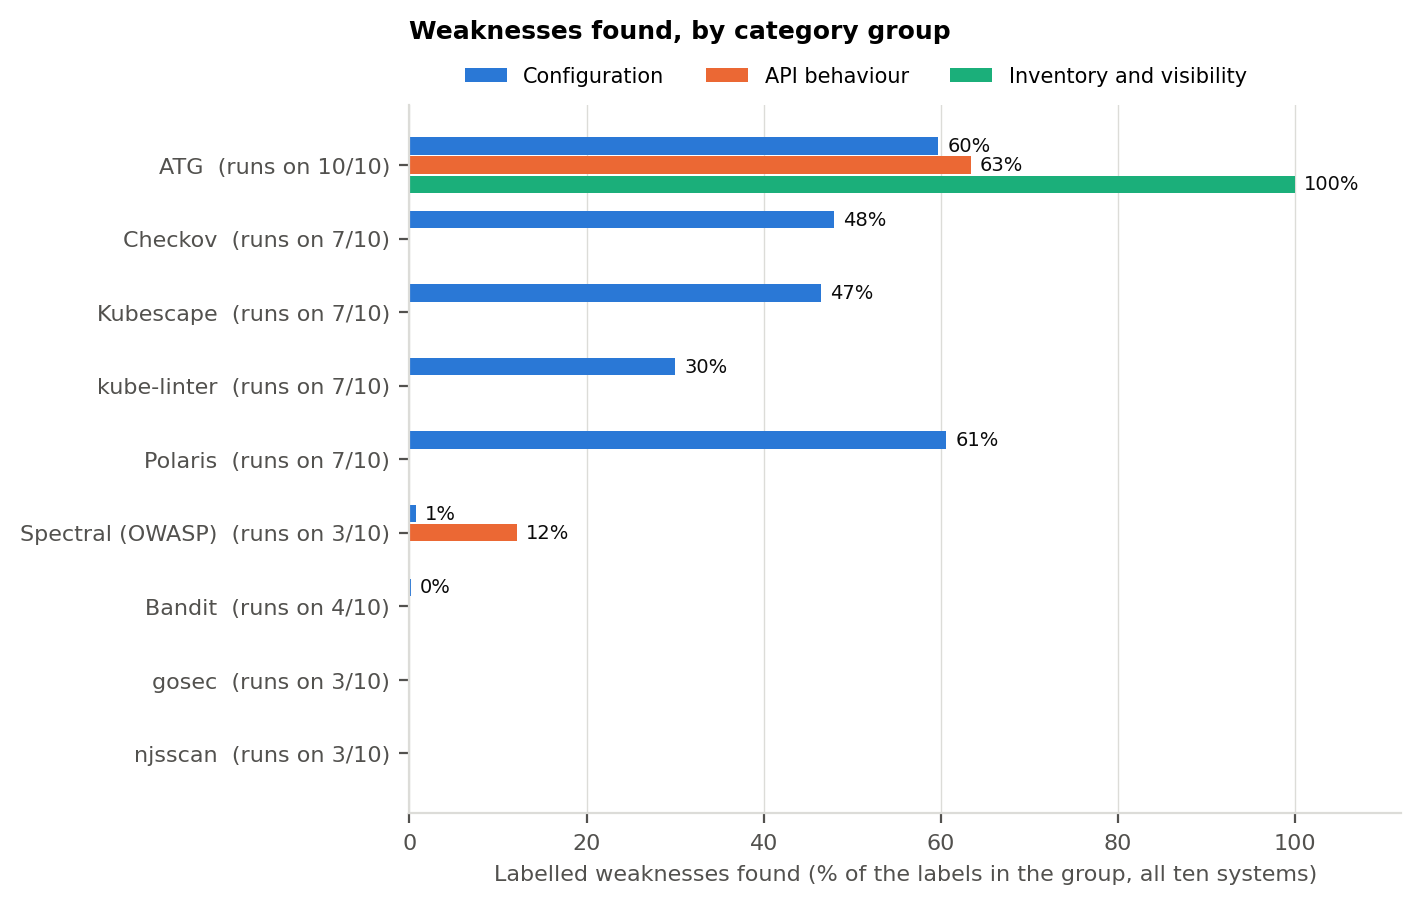
\includegraphics[width=0.7\textwidth]{figs/fig_oss_groups.png}
\caption{Labelled weaknesses found by category group on the ten open-source systems (716 labels); in brackets, the number of systems each tool can run on. Drawn by the benchmark script from the saved runs.}
\label{fig:tools}
\end{figure*}

\begin{figure*}[t]
\centering
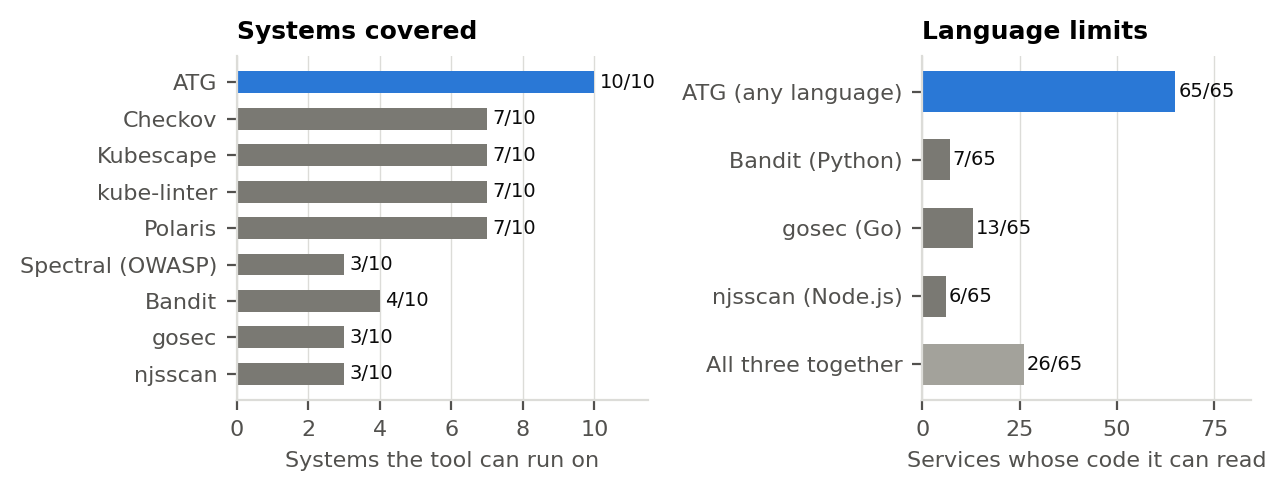
\includegraphics[width=0.8\textwidth]{figs/fig_oss_reach.png}
\caption{Where the other tools stop: systems each tool can run on (left) and services whose source code each single-language scanner can read (right).}
\label{fig:reach}
\end{figure*}

Every other tool stops at a coverage limit that ATG does not have (Fig.~\ref{fig:reach}). The four Kubernetes scanners cannot run on the three Compose systems, and Kubescape skipped FTGO's workloads because they use removed Kubernetes API versions. Spectral needs an API document, which seven of the ten systems do not have, and the documents that exist are incomplete: Bookinfo's lists 4 of its 13 operations. Each code scanner reads one language: Bandit could read 7 of the 65 services, gosec 13 and njsscan 6, so together they covered 26 services (40\%), and no free scanner here reads the Java, C\#, Ruby or PHP services. The code scanners found almost none of the labels, which is expected: they look for code flaws such as injection or weak cryptography, which none of the labels describe. ATG and a Kubernetes scanner complement each other. Together, ATG and Checkov find 613 of the 716 labels (86\%).

\textit{Baseline DAST comparison.} Table~\ref{tab:zap} compares ATG with OWASP ZAP on ShopLite. ZAP reached the 8 documented endpoints, sent 3,393 requests through the gateway in 27.7~s, and reported one valid low-risk issue (a missing \texttt{X-Content-Type-Options} header) and three informational alerts. It found none of the 40 planted weaknesses and none of the four shadow endpoints, which no document lists. ATG found 37 of 40, sending only 18 read-only requests of its own. ShopLite's weaknesses are design and deployment flaws and it has no injection flaws, which are the main strength of an active scanner. The two approaches are therefore complementary, and ATG's inventory, shadow endpoints included, can serve as the target list for an active scan.

\begin{table}[t]
\caption{ATG vs.\ OWASP ZAP 2.16.1 on ShopLite (vulnerable build)}
\label{tab:zap}
\centering
\footnotesize
\begin{tabular}{@{}lrrr@{}}
\toprule
 & ATG & ZAP (gateway) & ZAP (inside) \\
\midrule
Kind & passive & active & active \\
Requests sent to target & 18 & 3,393 & 3,527 \\
Time & 0.17 s* & 27.7 s & 16.7 s \\
Endpoints reached & 12/12 & 8/12 & 8/12 \\
Shadow endpoints found & 4/4 & 0/4 & 0/4 \\
Planted weaknesses found & 37/40 & 0/40 & 0/40 \\
Other valid issues & 0 & 1 & 1 \\
\bottomrule
\multicolumn{4}{@{}l}{\scriptsize *Phases 1--4 after the traffic was observed.}
\end{tabular}
\end{table}

\subsection{Attack-Path Risk Reduction and Remediation Impact}\label{sec:eval-c}
\textit{Measured reduction.} The hardened build of ShopLite implements the fixes the planner recommends, except two weaknesses kept on purpose: a deprecated endpoint still in use and an untraced cron job. Table~\ref{tab:hardening} compares the two builds under the same seeds. Under C1 the total attack-path risk falls from 467 to 13.5 (97.1\%), the attack paths from 121 to 2, and every run leaves only the two weaknesses kept on purpose. Under C2 the reduction is 94.5\%, and the remaining findings come from the services the experiment leaves untraced. The demonstration run shown in Figs.~\ref{fig:tg} and \ref{fig:fixcard} gives the same picture: 472 before and 13.5 after.

\begin{table}[t]
\caption{Applying the fixes: ShopLite vulnerable vs.\ hardened build (mean of five seeds)}
\label{tab:hardening}
\centering
\footnotesize
\begin{tabular}{@{}lrr@{}}
\toprule
 & C1 & C2 \\
\midrule
$R$ before $\rightarrow$ after & 467 $\rightarrow$ 13.5 & 405 $\rightarrow$ 22.1 \\
Measured reduction & 97.1\% & 94.5\% \\
Attack paths before $\rightarrow$ after & 121 $\rightarrow$ 2 & 108 $\rightarrow$ 4 \\
Findings after & 2.0 & 4.2 \\
Fixes the plan needs for 70\% of $R$ & 12.8 & 12.8 \\
\bottomrule
\end{tabular}
\end{table}

\textit{Concentration of risk.} APCR concentrates risk on a few fixes because a finding only counts through its best reachable path \eqref{eq:r}. On ShopLite, 13 of the planner's fixes remove 70\% of $R$ and 20 remove 90\%, although the scan reports 37 findings. On Train Ticket the plan needs 57 fixes for 70\% of $R$ under C1, against 231 findings, and on crAPI 31 fixes against 70 findings. Fig.~\ref{fig:plan} shows the planner's curve on the ten open-source systems, and Table~\ref{tab:plans} lists the numbers.

\begin{figure*}[t]
\centering
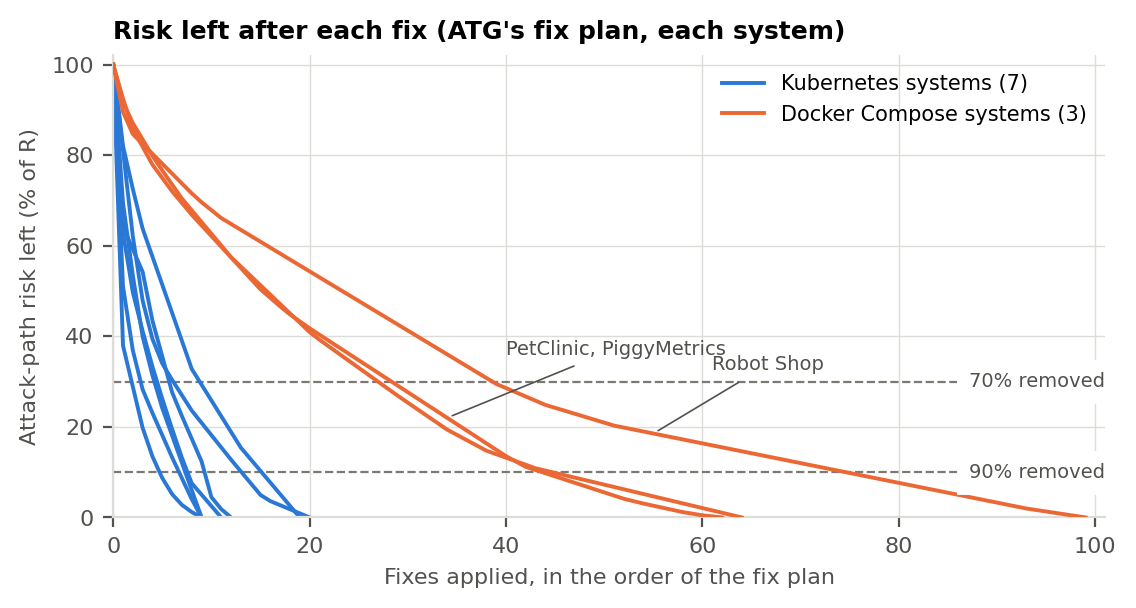
\includegraphics[width=0.7\textwidth]{figs/fig_oss_plans.png}
\caption{Attack-path risk left after each fix of ATG's plan, on the ten open-source systems.}
\label{fig:plan}
\end{figure*}

\begin{table}[t]
\caption{ATG's fix plan on the ten open-source systems}
\label{tab:plans}
\centering
\scriptsize
\setlength{\tabcolsep}{3pt}
\begin{tabular}{@{}lrrrrl@{}}
\toprule
System & Findings & $R$ & 70\% & 90\% & First fix \\
\midrule
Online Boutique & 97 & 380.0 & 6 & 10 & NetworkPolicy, frontend \\
Bank of Anthos & 45 & 173.5 & 3 & 7 & NetworkPolicy, frontend \\
Robot Shop$^{c}$ & 121 & 917.5 & 39 & 75 & route auth, \texttt{/api/cart/} \\
Acme Air & 143 & 443.0 & 7 & 14 & NetworkPolicy, booking \\
PetClinic$^{c}$ & 88 & 850.0 & 29 & 44 & route auth, \texttt{/api/customer} \\
PiggyMetrics$^{c}$ & 114 & 773.5 & 27 & 45 & route auth, \texttt{/accounts} \\
Lakeside Mutual & 118 & 414.5 & 5 & 8 & NetworkPolicy, policy backend \\
FTGO & 98 & 338.0 & 5 & 8 & NetworkPolicy, API gateway \\
Hotel Reservation & 113 & 331.0 & 9 & 16 & NetworkPolicy, frontend \\
Bookinfo & 32 & 126.5 & 2 & 5 & NetworkPolicy, productpage \\
\bottomrule
\multicolumn{6}{@{}l}{\scriptsize 70\%, 90\%: fixes needed to remove that share of $R$. $^{c}$Docker Compose.}
\end{tabular}
\end{table}

On the seven Kubernetes systems, 2--9 fixes remove 70\% of $R$, and the first fix is always a NetworkPolicy for the entry service: it cuts every in-cluster path that runs through that service, and on Bookinfo alone it removes 62\% of $R$. The three Compose systems need 27--39 fixes, because their risk is spread over many separate problems. In Robot Shop, 29 of the first 39 fixes document or remove an undocumented endpoint that is reachable from the internet; in PetClinic, ten stop publishing an internal server's port. The planner therefore also tells the reviewer what kind of work the system needs: one policy change, or a long list of small fixes.

\textit{From score to action.} The hardening report turns each step of the plan into work for the system's own stack (Fig.~\ref{fig:fixcard}). The fix for an unauthenticated route is written for the gateway that Phase 1 found. A NetworkPolicy lists exactly the callers the traces show, and a code fix names the finding's own operation. Each fix comes with a test that confirms it, for example ``call \texttt{GET /admin/transactions} as an ordinary user: expect 403''. Running the review again after the fix closes the loop, as the hardened ShopLite build shows.

\subsection{System Scalability and Graph Density Stress Testing}\label{sec:eval-d}
\textit{Per-system cost.} On the three oracle testbeds, Phase 2 normalization takes 3--30~ms and the rule engine 0.6--7~ms. A complete scan of an open-source system takes 7.2--8.1~s, of which Phases 1--4 take 0.2--0.9~s; most of the rest is a fixed wait for the sidecar and the Collector to go quiet before reading them. The recursive attack-path query on Train Ticket (1,006 paths) takes 6.5~s on SQLite and 54~ms on PostgreSQL, with identical results.

\textit{Stress test.} To find the limits, the EUJF of one ShopLite scan was cloned $k$ times behind one gateway ($k=1$ to 100), so that every copy carries real findings and paths. A second experiment kept 31 services and added $d$ random endpoint-to-endpoint calls per endpoint. Fig.~\ref{fig:stress} shows Phase~3 time on PostgreSQL. The test exposed two bottlenecks in version 1.2: the planner re-scored every action against every path at each step, so Phase~3 took 57~s at 61 services, and PostgreSQL planned the recursive query without table statistics. Version 1.3 scores an action only on the findings it touches and runs \texttt{ANALYZE} after loading the graph. It produces identical plans and paths, and it handles 301 services, 1,101 endpoints and 11,408 attack paths in 20.7~s with 226~MB of memory.

\begin{figure*}[t]
\centering
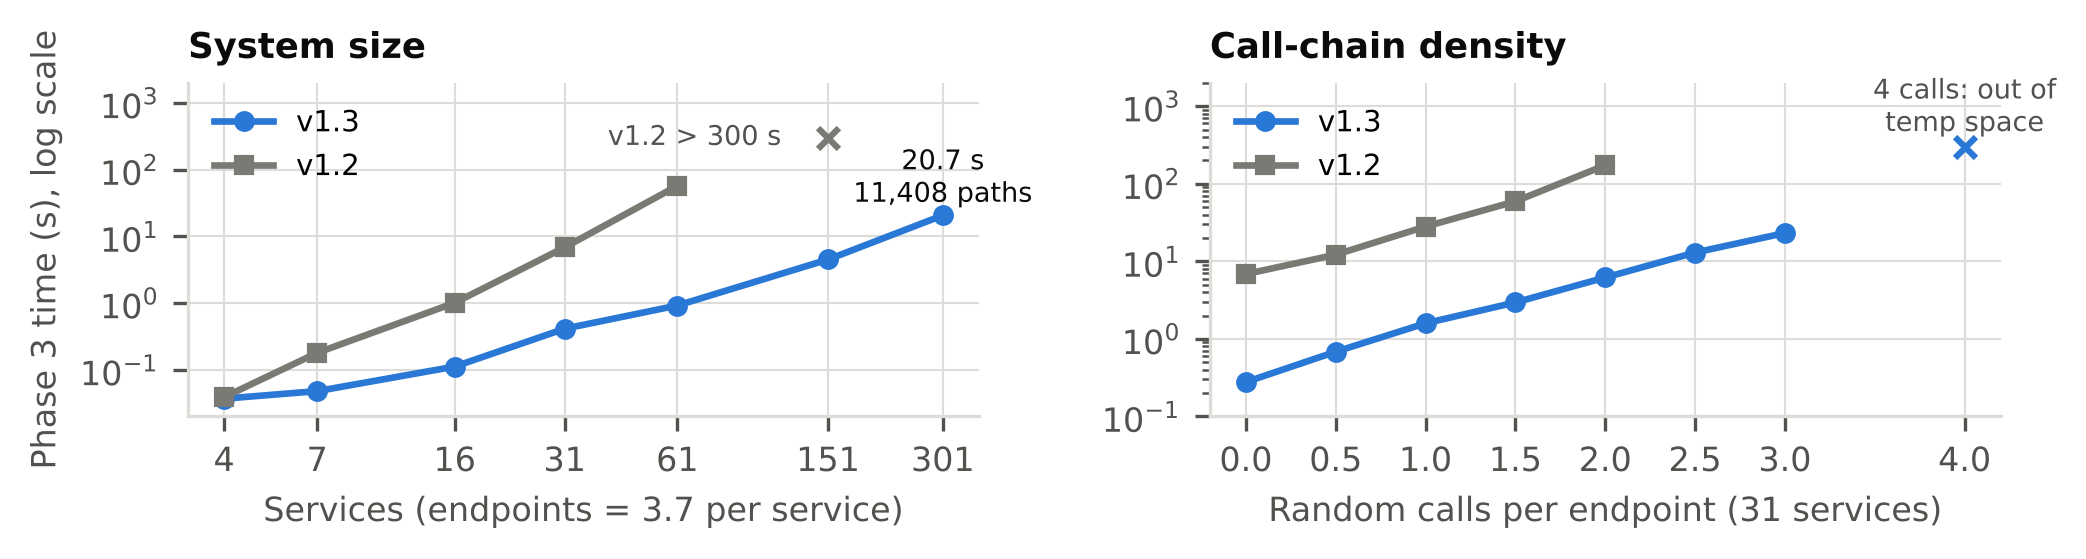
\includegraphics[width=0.82\textwidth]{figs/fig_stress.png}
\caption{Phase 3 time on PostgreSQL as the system grows (left) and as the call graph gets denser (right), versions 1.2 and 1.3.}
\label{fig:stress}
\end{figure*}

\textit{The remaining limit.} Call-chain density is the limit that remains. The query enumerates every simple path of up to nine hops, and their number grows exponentially with the number of calls per endpoint. With 31 services the analysis completes in 23~s at three calls per endpoint (12,813 paths) and exhausts 4~GB of temporary space at four. Since APCR keeps one best path per finding \eqref{eq:r}, a k-best-paths search would avoid the full enumeration. For comparison, the largest real system in our evaluation, Train Ticket, has 45 services. Capture volume is not a limit: twenty times the Train Ticket capture (160,220 flows and 260,200 spans) is processed in 17.4~s, and the inventory stays at exactly 220 entries.

\subsection{Negative Controls and Passive Detection Boundaries}\label{sec:eval-e}
\textit{Negative controls.} The ten generated companies contain 23 negative controls: configurations that a naive rule would flag but that are safe (Table~\ref{tab:controls}). Examples include a login protected by Kong's rate-limiting plugin, an nginx \texttt{limit\_req} directive or an Istio EnvoyFilter, an admin function that returns 403 to customers, routes behind an Istio ext-authz policy, and requests authenticated by a session cookie instead of a header. Version 1.3 flagged six of them. The fixes taught the extractor to read EnvoyFilter rate limits, Spring Cloud Gateway rate limiters, ext-authz policies and cookie credentials. Versions 1.4 and 1.5 flag none, while still finding the planted weaknesses (62 of 65).

\begin{table}[t]
\caption{Negative controls in the ten generated companies}
\label{tab:controls}
\centering
\footnotesize
\begin{tabular}{@{}p{2.6cm}rp{3.25cm}@{}}
\toprule
Rule a control tests & Controls & Safe because \\
\midrule
TS-07 login rate limit & 9 & limit in Kong, nginx, SCG, Istio EnvoyFilter, route table \\
API1 BOLA & 4 & owner check returns 403 \\
API5 admin function & 3 & role check returns 401 / 403 \\
TS-01, TS-02, TS-03 & 5 & cookie session, ext-authz, credential present \\
TS-08, API3 & 2 & STRICT mTLS; bulk data for keyed partners \\
\midrule
Flagged by v1.3 / v1.5 & 6 / 0 & \\
\bottomrule
\end{tabular}
\end{table}

\textit{What a passive review cannot see.} ATG never sends an attack request. This makes it safe to run next to a working system, and it also bounds what it can find. Table~\ref{tab:limits} summarizes the boundary by OWASP category. Of OWASP's 18 crAPI vulnerabilities, six need payload or model testing (NoSQL and SQL injection, JWT forgery, three LLM chatbot attacks) and are outside the scope of any passive review. Of the twelve in reach, four are flagged through another authorization rule, and the rest need response content, IDs in the query string or request semantics. No passive source shows those, and the stand-in replicas return generic bodies.

\begin{table*}[t]
\caption{Detection boundary by OWASP API Security Top 10 (2023) category}
\label{tab:limits}
\centering
\footnotesize
\begin{tabular}{@{}p{3.6cm}p{6.2cm}p{6.9cm}@{}}
\toprule
Category & What ATG detects & What it misses, and why \\
\midrule
API1 Object level authorization & object ID in the path, authenticated, never a 403 & IDs in query or body; cannot prove the hole without a second account \\
API2 Authentication & anonymous sensitive operations, unauthenticated routes, declared auth not enforced, credentials in URLs, logins without rate limit, unauthenticated service calls & weak secrets (values are never copied); token forgery \\
API3 Property level authorization & bulk sensitive data from anonymous or shadow endpoints & over-exposure to logged-in users; mass assignment (no rule) \\
API4 Resource consumption & internet-reachable services without limits; logins without rate limit & abuse through request content (repeat-count fields) \\
API5 Function level authorization & admin functions reachable by anonymous or ordinary callers & role gaps for logged-in users when anonymous calls get 401 \\
API6 Sensitive business flows & -- & needs business knowledge no source has \\
API7 SSRF & request fields typed or named as URLs & URL fields with other names (\texttt{photo\_url}, \texttt{mechanic\_api}) \\
API8 Misconfiguration & plaintext secrets, missing TLS, debug endpoints, root or privileged containers, NodePorts, missing NetworkPolicies, mutable tags & response headers, CORS; container hardening and service-account tokens (C9, C10) \\
API9 Inventory & shadow, zombie and undocumented services; untraced callers and workloads & endpoints never called during the review and in no document \\
API10 Unsafe consumption & third-party calls seen in traces & whether their responses are validated \\
Injection, LLM attacks & -- & need payloads: use an active scanner \\
\bottomrule
\end{tabular}
\end{table*}

\textit{Observation window.} Runtime sources see only what is used. Fig.~\ref{fig:curve} shows endpoint recall on Train Ticket as the workload grows. Traffic alone finds 32\% of the endpoints after 100 requests and 85\% after 4,000; with documents, manifests and traces added, recall is 96\% from the start.

\begin{figure}[t]
\centering
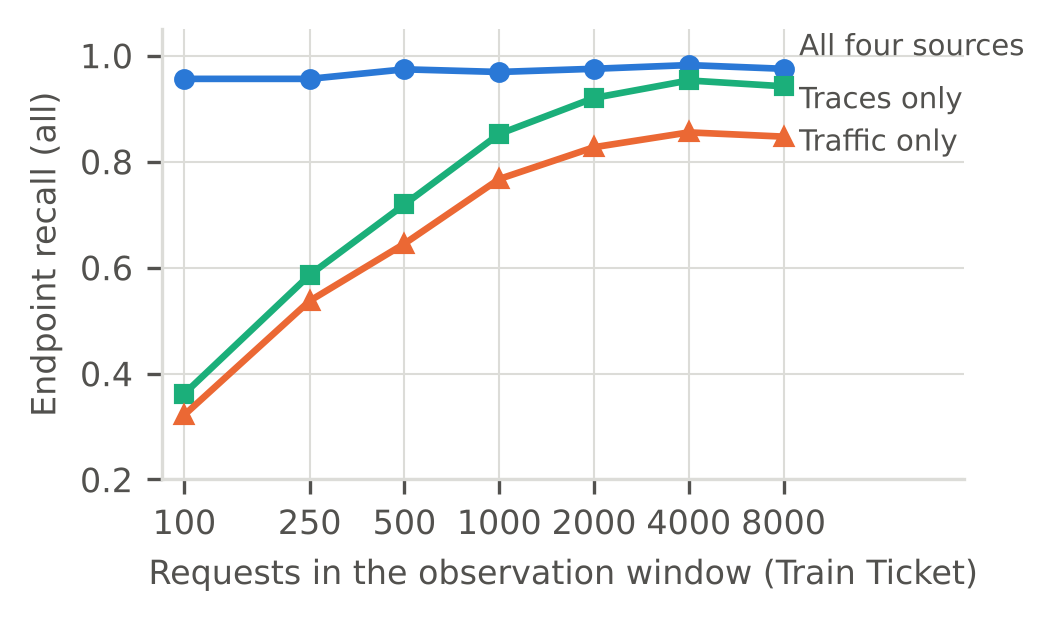
\includegraphics[width=\columnwidth]{figs/fig_curve.png}
\caption{Endpoint recall on Train Ticket as the observation window grows (condition C1, three seeds).}
\label{fig:curve}
\end{figure}

\textit{Misses on the open-source systems.} The largest gaps are exposed admin functions (1 of 7) and debug endpoints (2 of 7), whose paths (\texttt{/loader/load}, \texttt{/memory}) do not follow the naming the rules know, or which are whole consoles such as Spring Boot Admin, and missing resource limits (19 of 58), because ATG reports them only on internet-reachable services. These are known false negatives, which we report instead of tuning the rules to the labels.

\section{Discussion and Threats to Validity}\label{sec:discussion}
\textit{Stand-ins and replicas.} Train Ticket and crAPI ran as replicas, and the open-source systems ran as stand-ins, because the evaluation host could not pull container images. Both reproduce each system's operations, call graph and authentication but not its business logic, so rules that read response content fire less than they would on the real systems. The deployment files and API documents ATG read are the systems' own. The repository includes a kit that runs seven of the open-source systems on their published images.

\textit{Who wrote the ground truth.} ShopLite's planted list, the companies and the 91 hand-written labels were produced by the authors of the rules, which favours ATG. Two checks are independent of us: OWASP's crAPI list and the access-log ground truth of Group A. The rule-derived configuration labels resemble the checks of the Kubernetes scanners, which favours those scanners.

\textit{Tuning on the test systems.} The tool was changed during the evaluation. Four bugs were found in pilot runs and five by comparing the threat model with the oracle; the open-source systems then exposed five gaps in reading deployment files (Docker Compose, Zuul, multi-profile Spring Cloud Gateway files, Service and workload names, and TLS on entry points). All are general fixes. Version 1.4, before the open-source fixes, found 337 of the 716 labels (47\%) with 66\% precision; this is the fair estimate for systems the tool has never seen. Version 1.5 reaches 65\% and 75\%, and gives the same results as 1.4 on ShopLite and on the ten companies.

\textit{Mapping other tools.} Other tools' check identifiers were mapped to our categories by hand, so a real issue under an unmapped check counts as nothing. Commercial tools were compared only from their documentation. Performance was measured on one host with two vCPUs, so absolute times include CPU contention.

\section{Conclusion and Future Work}\label{sec:conclusion}
This paper presented ATG, a self-hosted platform for automatic API security design review of microservice systems. ATG combines runtime traffic, API documents, deployment and gateway configuration and distributed traces into one inventory, evaluates 27 deterministic rules, builds a threat graph and ranks attack paths with APCR. Combining the four sources found 97--100\% of observable endpoints at a precision of 1.00 where single sources reached 58--96\%. With full visibility, the threat model agreed with an oracle built from ground truth on every testbed. On ten published open-source systems, ATG found 65\% of 716 labelled weaknesses and ran on all ten. The best of eight free tools found 46\% and could not read three of the systems, and no other tool found API behaviour or inventory problems. ATG raised no alarm on 23 negative controls, and applying its planned fixes to the demonstration system removed 97\% of the attack-path risk.

Future work will run the open-source systems on their real images, add rules for mass assignment, query-parameter BOLA and container hardening, replace full path enumeration with a k-best-paths search to lift the density limit, and use ATG's inventory as the target list for an active scanner.

\begin{thebibliography}{99}
\bibitem{r1} A. M. Abdurrahman and E. Husni, ``A Secure Digital Image Marketplace: Microservices and OWASP API Security Using Spring Boot,'' in \textit{Proc. IEEE ICISS}, 2024, pp. 1--8.
\bibitem{r2} M. Idris, I. Syarif, and I. Winarno, ``Development of Vulnerable Web Application Based on OWASP API Security Risks,'' in \textit{Proc. IEEE IES}, 2021, pp. 190--194.
\bibitem{r3} M. George and S. Jonnalagadda, ``Enhancing API Security in Spring Boot Microservices using AI-based Threat Detection,'' in \textit{Proc. IEEE ICCBI}, 2026, pp. 637--642.
\bibitem{r4} Q. Tang, L. Ma, Z. Zhou, Z. Bu, and Y. Zhong, ``Formal Specification and Verification of API Security Based on Design by Contract,'' in \textit{Proc. IEEE ICPICS}, 2024, pp. 929--933.
\bibitem{r5} M. Sattanadin, ``Intelligent API Gateway Security Framework for Microservices using AI,'' in \textit{Proc. IEEE ICCMC}, 2026, pp. 2062--2068.
\bibitem{r6} J. A. D\'iaz-Rojas, J. O. Ochar\'an-Hern\'andez, J. C. P\'erez-Arriaga, and X. Lim\'on, ``Web API Security Vulnerabilities and Mitigation Mechanisms: A Systematic Mapping Study,'' in \textit{Proc. IEEE CONISOFT}, 2021, pp. 207--218.
\bibitem{r7} K. K. Ratra, D. K. Seth, D. Verma, and H. Burman, ``AI-Enhanced API Gateway: A Unified Framework for Security and Performance for Next Generation Microservices,'' in \textit{Proc. IEEE IEMCON}, 2025, pp. 577--584.
\bibitem{r8} N. Bhesaniya, D. Ladani, and S. Patel, ``Analysing API Access Behaviour for Enhanced Security: A Machine Learning Approach,'' in \textit{Proc. IEEE AIMV}, 2025, pp. 1--6.
\bibitem{r9} R. Sun, Q. Wang, and L. Guo, ``Research Towards Key Issues of API Security,'' in \textit{Proc. CNCERT}, 2022, pp. 179--192.
\bibitem{r10} NIST, ``Guide to Secure Web Services,'' NIST Special Publication 800-95, 2007.
\bibitem{owasp_api_2023} OWASP Foundation, ``OWASP API Security Top 10 -- 2023,'' 2023. [Online]. Available: \url{https://owasp.org/API-Security/editions/2023/en/0x00-header/}
\bibitem{nist_800_204} R. Chandramouli, ``Security Strategies for Microservices-based Application Systems,'' NIST Special Publication 800-204, 2019.
\bibitem{nist_800_207} S. Rose, O. Borchert, S. Mitchell, and S. Connelly, ``Zero Trust Architecture,'' NIST Special Publication 800-207, 2020.
\bibitem{checkov} Palo Alto Networks, ``Checkov: static analysis for infrastructure as code.'' [Online]. Available: \url{https://github.com/bridgecrewio/checkov}
\bibitem{kubescape} ARMO, ``Kubescape.'' [Online]. Available: \url{https://github.com/kubescape/kubescape}
\bibitem{polaris} Fairwinds, ``Polaris.'' [Online]. Available: \url{https://github.com/FairwindsOps/polaris}
\bibitem{spectral} Stoplight, ``Spectral'' and ``Spectral OWASP API Security ruleset.'' [Online]. Available: \url{https://github.com/stoplightio/spectral}
\bibitem{bandit} PyCQA, ``Bandit.'' [Online]. Available: \url{https://github.com/PyCQA/bandit}
\bibitem{gosec} Securego, ``gosec: Go security checker.'' [Online]. Available: \url{https://github.com/securego/gosec}
\bibitem{njsscan} A. Abraham, ``njsscan.'' [Online]. Available: \url{https://github.com/ajinabraham/njsscan}
\bibitem{zap} OWASP ZAP (Zed Attack Proxy). [Online]. Available: \url{https://www.zaproxy.org}
\bibitem{ibm_apic} IBM, ``Secure your APIs from design-time to run-time,'' IBM API Connect. [Online]. Available: \url{https://www.ibm.com/products/api-connect/secure}
\bibitem{salt} Salt Security, ``Salt Security announces API discovery updates for API Protection Platform,'' 2024. [Online]. Available: \url{https://www.securityinfowatch.com/cybersecurity/press-release/55131214/salt-security-announces-api-discovery-updates-for-api-protection-platform}
\bibitem{akamai_api} Akamai, ``Akamai API Security.'' [Online]. Available: \url{https://www.akamai.com/products/API-security}
\bibitem{shostack} A. Shostack, \textit{Threat Modeling: Designing for Security}. Indianapolis, IN, USA: Wiley, 2014.
\bibitem{ms_tmt} Microsoft, ``Understand threat modeling'' (Microsoft Threat Modeling Tool). [Online]. Available: \url{https://learn.microsoft.com/en-us/training/modules/introduction-to-secure-devops/7-understand-threat-modeling}
\bibitem{threat_dragon} OWASP Foundation, ``OWASP Threat Dragon.'' [Online]. Available: \url{https://owasp.org/projects/threat-dragon}
\bibitem{threagile} C. Schneider, ``Threagile: Agile threat modeling toolkit.'' [Online]. Available: \url{https://github.com/Threagile/threagile}
\bibitem{iriusrisk} IriusRisk, ``Infrastructure as code threat modeling.'' [Online]. Available: \url{https://iriusrisk.com/iac}
\bibitem{traceable} Harness, ``Harness and Traceable launch cloud-native security service for modern applications,'' 2025. [Online]. Available: \url{https://www.harness.io/press-and-news/harness-and-traceable-launch-cloud-native-security-service-for-modern-applications}
\bibitem{wiz} Google Cloud, ``Google completes acquisition of Wiz,'' 2026. [Online]. Available: \url{https://cloud.google.com/blog/products/identity-security/google-completes-acquisition-of-wiz}
\bibitem{prisma} Palo Alto Networks, ``Discover and protect API endpoints,'' Prisma Cloud documentation. [Online]. Available: \url{https://docs.prismacloud.io/use-cases/secure-the-infrastructure/discover-and-protect-api-endpoints}
\bibitem{defender_apis} Microsoft, ``Overview of Microsoft Defender for APIs.'' [Online]. Available: \url{https://learn.microsoft.com/azure/defender-for-cloud/defender-for-apis-introduction}
\bibitem{crunch42} 42Crunch, ``API Security Audit.'' [Online]. Available: \url{https://docs.42crunch.com/latest/content/concepts/api_contract_security_audit.htm}
\bibitem{morpheus} NVIDIA, ``NVIDIA Morpheus.'' [Online]. Available: \url{https://developer.nvidia.com/morpheus-cybersecurity}
\bibitem{kubelinter} StackRox (Red Hat), ``kube-linter.'' [Online]. Available: \url{https://github.com/stackrox/kube-linter}
\bibitem{graphml} U. Brandes, M. Eiglsperger, J. Lerner, and C. Pich, ``Graph Markup Language (GraphML),'' in \textit{Handbook of Graph Drawing and Visualization}, R. Tamassia, Ed. Boca Raton, FL, USA: CRC Press, 2013, pp. 517--541.
\bibitem{sarif} OASIS, ``Static Analysis Results Interchange Format (SARIF) Version 2.1.0,'' OASIS Standard, 2020.
\bibitem{mitmproxy} mitmproxy project, ``mitmproxy: an interactive HTTPS proxy.'' [Online]. Available: \url{https://mitmproxy.org}
\bibitem{otel} OpenTelemetry, ``OpenTelemetry specification.'' [Online]. Available: \url{https://opentelemetry.io/docs/specs/otel/}
\bibitem{attack} MITRE, ``ATT\&CK.'' [Online]. Available: \url{https://attack.mitre.org}
\bibitem{cwe} MITRE, ``Common Weakness Enumeration.'' [Online]. Available: \url{https://cwe.mitre.org}
\bibitem{nist_800_190} M. Souppaya, J. Morello, and K. Scarfone, ``Application Container Security Guide,'' NIST Special Publication 800-190, 2017.
\bibitem{trainticket} X. Zhou, X. Peng, T. Xie, J. Sun, C. Ji, W. Li, and D. Ding, ``Fault Analysis and Debugging of Microservice Systems: Industrial Survey, Benchmark System, and Empirical Study,'' \textit{IEEE Trans. Softw. Eng.}, vol. 47, no. 2, pp. 243--260, 2021.
\bibitem{crapi} OWASP Foundation, ``crAPI: completely ridiculous API.'' [Online]. Available: \url{https://github.com/OWASP/crAPI}
\bibitem{boutique} Google Cloud Platform, ``Online Boutique (microservices-demo),'' commit c7cb6d5. [Online]. Available: \url{https://github.com/GoogleCloudPlatform/microservices-demo}
\bibitem{anthos} Google Cloud Platform, ``Bank of Anthos,'' commit db35fea. [Online]. Available: \url{https://github.com/GoogleCloudPlatform/bank-of-anthos}
\bibitem{robotshop} Instana, ``Stan's Robot Shop,'' commit 55292e2. [Online]. Available: \url{https://github.com/instana/robot-shop}
\bibitem{acmeair} IBM blueperf, ``Acme Air microservices (Java),'' five repositories. [Online]. Available: \url{https://github.com/blueperf}
\bibitem{petclinic} Spring community, ``Spring PetClinic Microservices,'' commit e8b747a. [Online]. Available: \url{https://github.com/spring-petclinic/spring-petclinic-microservices}
\bibitem{piggymetrics} A. Lukyanchikov, ``PiggyMetrics,'' commit 6bb2cf9. [Online]. Available: \url{https://github.com/sqshq/piggymetrics}
\bibitem{lakeside} O. Zimmermann, M. Stocker, D. L\"ubke, U. Zdun, and C. Pautasso, \textit{Patterns for API Design: Simplifying Integration with Loosely Coupled Message Exchanges}. Addison-Wesley, 2022; sample application Lakeside Mutual, commit 357ca2d, \url{https://github.com/Microservice-API-Patterns/LakesideMutual}
\bibitem{ftgo} C. Richardson, \textit{Microservices Patterns}. Shelter Island, NY, USA: Manning, 2018; sample application FTGO, commit 558dfc5, \url{https://github.com/microservices-patterns/ftgo-application}
\bibitem{deathstarbench} Y. Gan \textit{et al.}, ``An Open-Source Benchmark Suite for Microservices and Their Hardware-Software Implications for Cloud \& Edge Systems,'' in \textit{Proc. ASPLOS}, 2019, pp. 3--18.
\bibitem{bookinfo} Istio project, ``Bookinfo sample application,'' commit 027bfe1. [Online]. Available: \url{https://github.com/istio/istio/tree/master/samples/bookinfo}
\end{thebibliography}

\end{document}
